% Options for packages loaded elsewhere
\PassOptionsToPackage{unicode}{hyperref}
\PassOptionsToPackage{hyphens}{url}
\PassOptionsToPackage{dvipsnames,svgnames,x11names}{xcolor}
%
\documentclass[
  a4paper,
  DIV=11,
  numbers=noendperiod,
  oneside]{scrartcl}

\usepackage{amsmath,amssymb}
\usepackage{setspace}
\usepackage{iftex}
\ifPDFTeX
  \usepackage[T1]{fontenc}
  \usepackage[utf8]{inputenc}
  \usepackage{textcomp} % provide euro and other symbols
\else % if luatex or xetex
  \usepackage{unicode-math}
  \defaultfontfeatures{Scale=MatchLowercase}
  \defaultfontfeatures[\rmfamily]{Ligatures=TeX,Scale=1}
\fi
\usepackage{lmodern}
\ifPDFTeX\else  
    % xetex/luatex font selection
\fi
% Use upquote if available, for straight quotes in verbatim environments
\IfFileExists{upquote.sty}{\usepackage{upquote}}{}
\IfFileExists{microtype.sty}{% use microtype if available
  \usepackage[]{microtype}
  \UseMicrotypeSet[protrusion]{basicmath} % disable protrusion for tt fonts
}{}
\makeatletter
\@ifundefined{KOMAClassName}{% if non-KOMA class
  \IfFileExists{parskip.sty}{%
    \usepackage{parskip}
  }{% else
    \setlength{\parindent}{0pt}
    \setlength{\parskip}{6pt plus 2pt minus 1pt}}
}{% if KOMA class
  \KOMAoptions{parskip=half}}
\makeatother
\usepackage{xcolor}
\usepackage[top=2cm,bottom=4cm,left=2cm,right=2cm,heightrounded]{geometry}
\setlength{\emergencystretch}{3em} % prevent overfull lines
\setcounter{secnumdepth}{-\maxdimen} % remove section numbering
% Make \paragraph and \subparagraph free-standing
\makeatletter
\ifx\paragraph\undefined\else
  \let\oldparagraph\paragraph
  \renewcommand{\paragraph}{
    \@ifstar
      \xxxParagraphStar
      \xxxParagraphNoStar
  }
  \newcommand{\xxxParagraphStar}[1]{\oldparagraph*{#1}\mbox{}}
  \newcommand{\xxxParagraphNoStar}[1]{\oldparagraph{#1}\mbox{}}
\fi
\ifx\subparagraph\undefined\else
  \let\oldsubparagraph\subparagraph
  \renewcommand{\subparagraph}{
    \@ifstar
      \xxxSubParagraphStar
      \xxxSubParagraphNoStar
  }
  \newcommand{\xxxSubParagraphStar}[1]{\oldsubparagraph*{#1}\mbox{}}
  \newcommand{\xxxSubParagraphNoStar}[1]{\oldsubparagraph{#1}\mbox{}}
\fi
\makeatother

\usepackage{color}
\usepackage{fancyvrb}
\newcommand{\VerbBar}{|}
\newcommand{\VERB}{\Verb[commandchars=\\\{\}]}
\DefineVerbatimEnvironment{Highlighting}{Verbatim}{commandchars=\\\{\}}
% Add ',fontsize=\small' for more characters per line
\usepackage{framed}
\definecolor{shadecolor}{RGB}{241,243,245}
\newenvironment{Shaded}{\begin{snugshade}}{\end{snugshade}}
\newcommand{\AlertTok}[1]{\textcolor[rgb]{0.68,0.00,0.00}{#1}}
\newcommand{\AnnotationTok}[1]{\textcolor[rgb]{0.37,0.37,0.37}{#1}}
\newcommand{\AttributeTok}[1]{\textcolor[rgb]{0.40,0.45,0.13}{#1}}
\newcommand{\BaseNTok}[1]{\textcolor[rgb]{0.68,0.00,0.00}{#1}}
\newcommand{\BuiltInTok}[1]{\textcolor[rgb]{0.00,0.23,0.31}{#1}}
\newcommand{\CharTok}[1]{\textcolor[rgb]{0.13,0.47,0.30}{#1}}
\newcommand{\CommentTok}[1]{\textcolor[rgb]{0.37,0.37,0.37}{#1}}
\newcommand{\CommentVarTok}[1]{\textcolor[rgb]{0.37,0.37,0.37}{\textit{#1}}}
\newcommand{\ConstantTok}[1]{\textcolor[rgb]{0.56,0.35,0.01}{#1}}
\newcommand{\ControlFlowTok}[1]{\textcolor[rgb]{0.00,0.23,0.31}{\textbf{#1}}}
\newcommand{\DataTypeTok}[1]{\textcolor[rgb]{0.68,0.00,0.00}{#1}}
\newcommand{\DecValTok}[1]{\textcolor[rgb]{0.68,0.00,0.00}{#1}}
\newcommand{\DocumentationTok}[1]{\textcolor[rgb]{0.37,0.37,0.37}{\textit{#1}}}
\newcommand{\ErrorTok}[1]{\textcolor[rgb]{0.68,0.00,0.00}{#1}}
\newcommand{\ExtensionTok}[1]{\textcolor[rgb]{0.00,0.23,0.31}{#1}}
\newcommand{\FloatTok}[1]{\textcolor[rgb]{0.68,0.00,0.00}{#1}}
\newcommand{\FunctionTok}[1]{\textcolor[rgb]{0.28,0.35,0.67}{#1}}
\newcommand{\ImportTok}[1]{\textcolor[rgb]{0.00,0.46,0.62}{#1}}
\newcommand{\InformationTok}[1]{\textcolor[rgb]{0.37,0.37,0.37}{#1}}
\newcommand{\KeywordTok}[1]{\textcolor[rgb]{0.00,0.23,0.31}{\textbf{#1}}}
\newcommand{\NormalTok}[1]{\textcolor[rgb]{0.00,0.23,0.31}{#1}}
\newcommand{\OperatorTok}[1]{\textcolor[rgb]{0.37,0.37,0.37}{#1}}
\newcommand{\OtherTok}[1]{\textcolor[rgb]{0.00,0.23,0.31}{#1}}
\newcommand{\PreprocessorTok}[1]{\textcolor[rgb]{0.68,0.00,0.00}{#1}}
\newcommand{\RegionMarkerTok}[1]{\textcolor[rgb]{0.00,0.23,0.31}{#1}}
\newcommand{\SpecialCharTok}[1]{\textcolor[rgb]{0.37,0.37,0.37}{#1}}
\newcommand{\SpecialStringTok}[1]{\textcolor[rgb]{0.13,0.47,0.30}{#1}}
\newcommand{\StringTok}[1]{\textcolor[rgb]{0.13,0.47,0.30}{#1}}
\newcommand{\VariableTok}[1]{\textcolor[rgb]{0.07,0.07,0.07}{#1}}
\newcommand{\VerbatimStringTok}[1]{\textcolor[rgb]{0.13,0.47,0.30}{#1}}
\newcommand{\WarningTok}[1]{\textcolor[rgb]{0.37,0.37,0.37}{\textit{#1}}}

\providecommand{\tightlist}{%
  \setlength{\itemsep}{0pt}\setlength{\parskip}{0pt}}\usepackage{longtable,booktabs,array}
\usepackage{calc} % for calculating minipage widths
% Correct order of tables after \paragraph or \subparagraph
\usepackage{etoolbox}
\makeatletter
\patchcmd\longtable{\par}{\if@noskipsec\mbox{}\fi\par}{}{}
\makeatother
% Allow footnotes in longtable head/foot
\IfFileExists{footnotehyper.sty}{\usepackage{footnotehyper}}{\usepackage{footnote}}
\makesavenoteenv{longtable}
\usepackage{graphicx}
\makeatletter
\def\maxwidth{\ifdim\Gin@nat@width>\linewidth\linewidth\else\Gin@nat@width\fi}
\def\maxheight{\ifdim\Gin@nat@height>\textheight\textheight\else\Gin@nat@height\fi}
\makeatother
% Scale images if necessary, so that they will not overflow the page
% margins by default, and it is still possible to overwrite the defaults
% using explicit options in \includegraphics[width, height, ...]{}
\setkeys{Gin}{width=\maxwidth,height=\maxheight,keepaspectratio}
% Set default figure placement to htbp
\makeatletter
\def\fps@figure{htbp}
\makeatother
% definitions for citeproc citations
\NewDocumentCommand\citeproctext{}{}
\NewDocumentCommand\citeproc{mm}{%
  \begingroup\def\citeproctext{#2}\cite{#1}\endgroup}
\makeatletter
 % allow citations to break across lines
 \let\@cite@ofmt\@firstofone
 % avoid brackets around text for \cite:
 \def\@biblabel#1{}
 \def\@cite#1#2{{#1\if@tempswa , #2\fi}}
\makeatother
\newlength{\cslhangindent}
\setlength{\cslhangindent}{1.5em}
\newlength{\csllabelwidth}
\setlength{\csllabelwidth}{3em}
\newenvironment{CSLReferences}[2] % #1 hanging-indent, #2 entry-spacing
 {\begin{list}{}{%
  \setlength{\itemindent}{0pt}
  \setlength{\leftmargin}{0pt}
  \setlength{\parsep}{0pt}
  % turn on hanging indent if param 1 is 1
  \ifodd #1
   \setlength{\leftmargin}{\cslhangindent}
   \setlength{\itemindent}{-1\cslhangindent}
  \fi
  % set entry spacing
  \setlength{\itemsep}{#2\baselineskip}}}
 {\end{list}}
\usepackage{calc}
\newcommand{\CSLBlock}[1]{\hfill\break\parbox[t]{\linewidth}{\strut\ignorespaces#1\strut}}
\newcommand{\CSLLeftMargin}[1]{\parbox[t]{\csllabelwidth}{\strut#1\strut}}
\newcommand{\CSLRightInline}[1]{\parbox[t]{\linewidth - \csllabelwidth}{\strut#1\strut}}
\newcommand{\CSLIndent}[1]{\hspace{\cslhangindent}#1}

\KOMAoption{captions}{tableheading}
\makeatletter
\@ifpackageloaded{caption}{}{\usepackage{caption}}
\AtBeginDocument{%
\ifdefined\contentsname
  \renewcommand*\contentsname{Indholdsfortegnelse}
\else
  \newcommand\contentsname{Indholdsfortegnelse}
\fi
\ifdefined\listfigurename
  \renewcommand*\listfigurename{Figuroversigt}
\else
  \newcommand\listfigurename{Figuroversigt}
\fi
\ifdefined\listtablename
  \renewcommand*\listtablename{Tabeloversigt}
\else
  \newcommand\listtablename{Tabeloversigt}
\fi
\ifdefined\figurename
  \renewcommand*\figurename{Figur}
\else
  \newcommand\figurename{Figur}
\fi
\ifdefined\tablename
  \renewcommand*\tablename{Tabel}
\else
  \newcommand\tablename{Tabel}
\fi
}
\@ifpackageloaded{float}{}{\usepackage{float}}
\floatstyle{ruled}
\@ifundefined{c@chapter}{\newfloat{codelisting}{h}{lop}}{\newfloat{codelisting}{h}{lop}[chapter]}
\floatname{codelisting}{Liste}
\newcommand*\listoflistings{\listof{codelisting}{Listeoversigt}}
\makeatother
\makeatletter
\makeatother
\makeatletter
\@ifpackageloaded{caption}{}{\usepackage{caption}}
\@ifpackageloaded{subcaption}{}{\usepackage{subcaption}}
\makeatother
\makeatletter
\@ifpackageloaded{sidenotes}{}{\usepackage{sidenotes}}
\@ifpackageloaded{marginnote}{}{\usepackage{marginnote}}
\makeatother

\ifLuaTeX
\usepackage[bidi=basic]{babel}
\else
\usepackage[bidi=default]{babel}
\fi
\babelprovide[main,import]{danish}
% get rid of language-specific shorthands (see #6817):
\let\LanguageShortHands\languageshorthands
\def\languageshorthands#1{}
\ifLuaTeX
  \usepackage{selnolig}  % disable illegal ligatures
\fi
\usepackage{bookmark}

\IfFileExists{xurl.sty}{\usepackage{xurl}}{} % add URL line breaks if available
\urlstyle{same} % disable monospaced font for URLs
\hypersetup{
  pdftitle={Nemt Danmarkskort i R},
  pdfauthor={Aleksander Bang-Larsen},
  pdflang={da},
  colorlinks=true,
  linkcolor={blue},
  filecolor={Maroon},
  citecolor={Blue},
  urlcolor={Blue},
  pdfcreator={LaTeX via pandoc}}


\title{Nemt Danmarkskort i R}
\author{Aleksander Bang-Larsen}
\date{2024-06-29}

\begin{document}
\maketitle

\renewcommand*\contentsname{Indholdsfortegnelse}
{
\hypersetup{linkcolor=}
\setcounter{tocdepth}{3}
\tableofcontents
}

\setstretch{1.5}
\subsection{Baggrund}\label{baggrund}

Da jeg skulle lære at lave kort i R, lavede jeg et par hurtige
googlesøgninger, hvor jeg kom frem til en god guide lavet af Mikkel
Freltoft Krogsholm (2021). Jeg opdagede dog hurtigt, at guiden er
out-of-date - og derfor skriver jeg denne guide.

I denne guide vil jeg gennemgå hvordan man kan skabe et kort over alle
afstemningssteders områder i Danmark. Vi vil både producere et kort for
Aarhus Kommune (Figur~\ref{fig-aarhus}) og et kort for alle
afstemningsområder i hele Danmark (Figur~\ref{fig-dk}).

\subsection{Pakker}\label{pakker}

I R-universet findes der flere pakker til at arbejde med kort. Jeg har
valgt at bruge \texttt{\{sf\}}som den pakke jeg sætter mig ind i, hvad
kan. De fleste kan grundlæggende det samme og er bygget op omkring
\texttt{geometry}, der er den kolonne (eller variabel) i en dataframe,
der indeholder figurerne til kortet.

Først indlæser vi alle pakker der skal bruges.

\begin{Shaded}
\begin{Highlighting}[]
\FunctionTok{library}\NormalTok{(tidyverse)      }\CommentTok{\# Her får vi \%\textgreater{}\%, ggplot2 og andre smarte funktioner.}
\FunctionTok{library}\NormalTok{(sf)             }\CommentTok{\# Skal bruges til at arbejde med "simple features" (figurer).}
\end{Highlighting}
\end{Shaded}

\subsection{Data}\label{data}

For at tegne et præcist danmarkskort kan vi hente \texttt{geojson} data
fra Styrelsen for Dataforsyning og Infrastruktur (2024). De udstiller en
udmærket \texttt{API} der kan levere kortdata til os. For at vi kan
benytte en \texttt{API} i \texttt{R} skal vi først definere et
\texttt{URL} og dernæst bede om at downloade den fil der hører til på
den hjemmeside.

\begin{enumerate}
\def\labelenumi{\arabic{enumi}.}
\tightlist
\item
  Først definerer vi \texttt{API}ens \texttt{URL}.
\end{enumerate}

\begin{Shaded}
\begin{Highlighting}[]
\DocumentationTok{\#\# Gemmer URL til API{-}kald}
\NormalTok{url }\OtherTok{\textless{}{-}} \StringTok{"https://api.dataforsyningen.dk/afstemningsomraader?format=geojson"}
\end{Highlighting}
\end{Shaded}

\marginnote{\begin{footnotesize}

Du behøver \emph{ikke} at vide hvad en \texttt{API} er for at kunne
gennemføre denne guide.

\end{footnotesize}}

\begin{enumerate}
\def\labelenumi{\arabic{enumi}.}
\setcounter{enumi}{1}
\tightlist
\item
  Dernæst beder vi \texttt{R} om at downloade den efterspurgte fil til
  en midlertidig placering i computerens hukommelse.
\end{enumerate}

\begin{Shaded}
\begin{Highlighting}[]
\CommentTok{\# Skaber midlertidig fil}
\NormalTok{geofile }\OtherTok{\textless{}{-}} \FunctionTok{tempfile}\NormalTok{()}

\CommentTok{\# Henter geojson til tempfile}
\FunctionTok{download.file}\NormalTok{(url, geofile)}
\end{Highlighting}
\end{Shaded}

Vi bruger funktionen \texttt{download.file()} og giver den
\texttt{API}ens \texttt{URL} og den midlertidige dataplacering, hvor vi
ønsker dataene hentet til.

\begin{enumerate}
\def\labelenumi{\arabic{enumi}.}
\setcounter{enumi}{2}
\tightlist
\item
  Til sidst omformer vi \texttt{geoJSON} til et \texttt{sf} format som
  \texttt{R} kan forstå.
\end{enumerate}

\begin{Shaded}
\begin{Highlighting}[]
\CommentTok{\# Læser datafilen ind i R}
\NormalTok{geodata\_st }\OtherTok{\textless{}{-}} \FunctionTok{st\_read}\NormalTok{(geofile)}
\NormalTok{afstemningssteder\_geodata }\OtherTok{\textless{}{-}} \FunctionTok{st\_as\_sf}\NormalTok{(geodata\_st)}
\end{Highlighting}
\end{Shaded}

\marginnote{\begin{footnotesize}

Her omformes først til \texttt{st} og dernæst til \texttt{sf}.

\end{footnotesize}}

Nu har vi en dataframe i \texttt{afstemningssteder\_geodata} der
indeholder de figurer vi skal bruge for at lave et danmarkskort!

\subsubsection{Optimering af data}\label{optimering-af-data}

For at vi nemt kan rendere vores plots er det en god ide at gøre
figurerne en smule mindre. \emph{Især} når vi er helt nede på
afstemningsstedsniveau. Det er nok ikke så relevant, hvis vi arbejder
med kommuner eller landsdele.

\begin{Shaded}
\begin{Highlighting}[]
\NormalTok{afstemningssteder\_geodata }\OtherTok{\textless{}{-}}\NormalTok{ rmapshaper}\SpecialCharTok{::}\FunctionTok{ms\_simplify}\NormalTok{(afstemningssteder\_geodata,}
                                                     \AttributeTok{keep =} \FloatTok{0.01}\NormalTok{, }\AttributeTok{keep\_shapes =} \ConstantTok{TRUE}\NormalTok{)}
\end{Highlighting}
\end{Shaded}

\marginnote{\begin{footnotesize}

Her indlæser vi \texttt{rmapshaper::ms\_simplify()} med pakkens navn for
at slippe for at indlæse hele pakken - Vi skal nemlig ikke bruge det
hele! Det samme har vi gjort med \texttt{ggthemes::theme\_map()}
nedenfor, fordi der kun skal bruges det ene \emph{theme}

\end{footnotesize}}

\subsection{Visualisering}\label{visualisering}

Nu kommer vi til den sjove del - At lave selve kortet! Vi skal bruge
\texttt{\{ggplot2\}} fra det velkendte \emph{tidyverse}, præcis som når
vi laver grafer i mange andre sammenhænge.

Vi bruger \texttt{geom\_sf}, der er indbygget i \texttt{\{ggplot2\}} til
at tegne de figurer der er opbevaret i vores dataframe. Jeg putter
derudover også \texttt{ggthemes::theme\_map()} på, fordi jeg ikke synes
kort behøver akselinjer og en baggrund. \texttt{theme\_map()} er mit
klart foretrukne tema til kort.

\begin{Shaded}
\begin{Highlighting}[]
\FunctionTok{ggplot}\NormalTok{(afstemningssteder\_geodata) }\SpecialCharTok{+}
  \FunctionTok{geom\_sf}\NormalTok{() }\SpecialCharTok{+}
\NormalTok{  ggthemes}\SpecialCharTok{::}\FunctionTok{theme\_map}\NormalTok{() }\SpecialCharTok{+}
  \FunctionTok{labs}\NormalTok{(}\AttributeTok{title =} \StringTok{"Afstemningssteder i Danmark"}\NormalTok{,}
       \AttributeTok{caption =} \StringTok{"Kilde: DAWA/DAGI"}\NormalTok{) }\SpecialCharTok{+}
  \FunctionTok{theme}\NormalTok{(}\AttributeTok{legend.position =} \StringTok{"none"}\NormalTok{,}
        \AttributeTok{plot.title =} \FunctionTok{element\_text}\NormalTok{(}\AttributeTok{size =} \DecValTok{20}\NormalTok{),}
        \AttributeTok{plot.caption =} \FunctionTok{element\_text}\NormalTok{(}\AttributeTok{size =} \DecValTok{10}\NormalTok{))}
\end{Highlighting}
\end{Shaded}

{
\makeatletter
\def\LT@makecaption#1#2#3{%
  \noalign{\smash{\hbox{\kern\textwidth\rlap{\kern\marginparsep
  \parbox[t]{\marginparwidth}{%
    \footnotesize{%
      \vspace{(1.1\baselineskip)}
    #1{#2: }\ignorespaces #3}}}}}}%
    }
\makeatother

\begin{figure}[H]

\sidecaption{\label{fig-dk}Kort over alle afstemningsområder i hele
Danmark. Kilde og titel tilføjet.}

\centering{

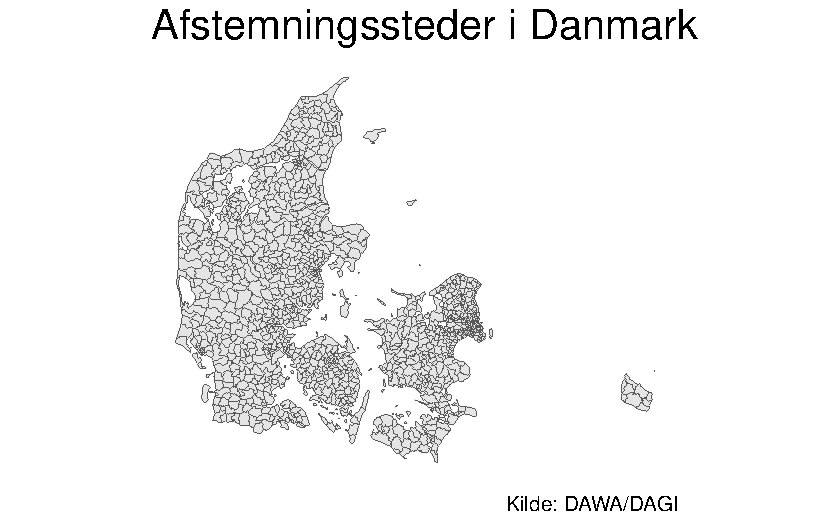
\includegraphics{index_files/figure-pdf/fig-dk-1.pdf}

}

\end{figure}%

}

\subsubsection{Visualisering af udsnit}\label{visualisering-af-udsnit}

For at kun vise de afstemningsområder der ligger i Aarhus Kommune kan vi
benytte os af \texttt{filter()} funktionen fra \texttt{\{dplyr\}}
pakken. Med den kan vi filtrere i vores dataframe, så der kun vises
afstemningssteder, hvor kommunenavnet er ``Aarhus''. Derudover har jeg
tilføjet et \texttt{fill} på afstemningsområdets navn for at give hver
område sin egen farve.

\begin{Shaded}
\begin{Highlighting}[]
\NormalTok{afstemningssteder\_geodata }\SpecialCharTok{\%\textgreater{}\%}
  \FunctionTok{filter}\NormalTok{(kommunenavn }\SpecialCharTok{==} \StringTok{"Aarhus"}\NormalTok{) }\SpecialCharTok{\%\textgreater{}\%}
  \FunctionTok{ggplot}\NormalTok{(}\FunctionTok{aes}\NormalTok{(}\AttributeTok{fill =}\NormalTok{ navn)) }\SpecialCharTok{+}
  \FunctionTok{geom\_sf}\NormalTok{() }\SpecialCharTok{+}
\NormalTok{  ggthemes}\SpecialCharTok{::}\FunctionTok{theme\_map}\NormalTok{() }\SpecialCharTok{+}
  \FunctionTok{theme}\NormalTok{(}\AttributeTok{legend.position =} \StringTok{"none"}\NormalTok{)}
\end{Highlighting}
\end{Shaded}

{
\makeatletter
\def\LT@makecaption#1#2#3{%
  \noalign{\smash{\hbox{\kern\textwidth\rlap{\kern\marginparsep
  \parbox[t]{\marginparwidth}{%
    \footnotesize{%
      \vspace{(1.1\baselineskip)}
    #1{#2: }\ignorespaces #3}}}}}}%
    }
\makeatother

\begin{figure}[H]

\sidecaption{\label{fig-aarhus}Kort over alle afstemningsområder i
Aarhus Kommune.}

\centering{

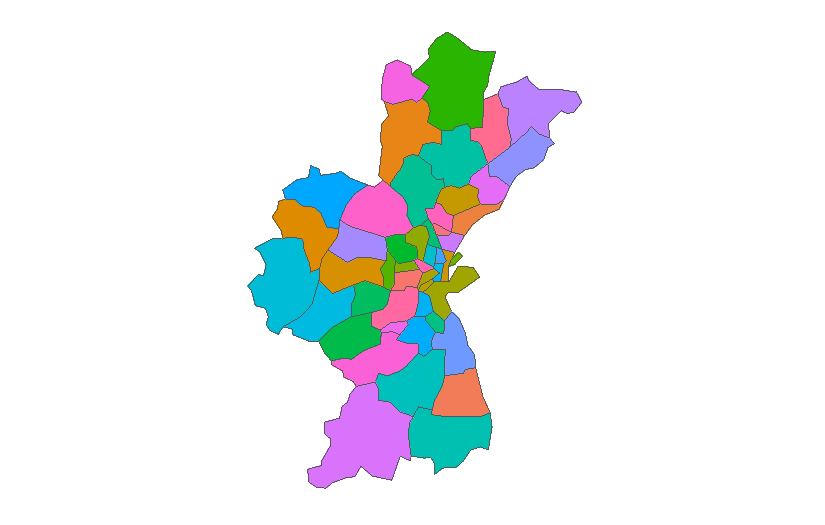
\includegraphics{index_files/figure-pdf/fig-aarhus-1.pdf}

}

\end{figure}%

}

\subsection{Samlet kode}\label{samlet-kode}

Alt hvad jeg har gennemgået i denne guide kan findes i et samlet
\texttt{r}-script
\href{https://github.com/aleksanderbl29/aleksanderbldk/blob/main/guides/2024-06-29-danmarkskort-i-r/kort.r}{på
min github}. Den kan også findes \href{./kort-kode.qmd}{her på
hjemmesiden}.

\phantomsection\label{refs}
\begin{CSLReferences}{1}{0}
\bibitem[\citeproctext]{ref-krogsholm2021}
Krogsholm, Mikkel Freltoft. 2021. {``Easy Maps of {Denmark} in {R}
{\textbar} {LinkedIn}''}.
https://www.linkedin.com/pulse/easy-maps-denmark-r-mikkel-freltoft-krogsholm/.

\bibitem[\citeproctext]{ref-apidawa2024}
Styrelsen for Dataforsyning og Infrastruktur. 2024. {``{DAWA}: {Danmarks
Adressers Web API} Hos {Dataforsyningen}''}.
https://dawadocs.dataforsyningen.dk/dok/guides.

\end{CSLReferences}




\end{document}
